\section{Evaluation} \label{sec_05}
In diesem Abschnitt wird die durchgeführte Arbeit überprüft. Hierbei wird bestimmt, ob die Anforderungen erfüllt wurden, wie sorgfältig der Code geschrieben wurde, wie geeignet die gewählten Technologien sind und inwiefern auf dem Projekt aufgebaut werden kann.

\subsection{Anforderungen}
Im Folgenden wird untersucht, ob die in Abschnitt 3 gestellten Anforderungen vom Projekt erfüllt werden.

\paragraph{Automatischer Start und Sprachsteuerung}
Das System verbindet sich nach dem Start automatisch mit den Diensten, es bedarf keinen weiteren Eingaben des Nutzenden. Um mit dem System zu interagieren benötigt der Nutzende lediglich den Sprachassistenten, über diesen kann er weitere Informationen erhalten und nach Hilfe fragen.

\paragraph{Informationsabfrage in unter drei Sekunden}
Die Reaktionszeiten des Systems sind sehr gut, von Anfrage bis Reaktion vergeht nur eine Sekunde:

\begin{verbatim}
    2024-05-31 13:08:43 server-1    | root - INFO - Retrieving
        Data from InfluxDB
    2024-05-31 13:08:44 server-1    | root - INFO - Plant environment: 
        Time: 2024-05-31 
        11:08:44.570381, 
        Temperature: 21.0, 
        Light: 609.9333333333333, 
        Humidity: 57.666666666666664, 
        Moisture: 37.6
    2024-05-31 13:08:44 server-1    | root - DEBUG - Searching for plant 
        'Succulent'.
    2024-05-31 13:08:44 server-1    | root - INFO - Comparing sensor data 
        with optimal values
    2024-05-31 13:08:44 server-1    | root - INFO - Soil Moisture
        adequate.
\end{verbatim}

\paragraph{Senden der Daten jede Minute, Überprüfen der Daten alle fünf Minuten}
Die Threads den Main Controllers und des Mikrocontrollers, sind so gestaltet, dass jede Minute die Sensorwerte gesendet werden, und alle fünf Minuten, die Werte der letzten fünf Minuten ausgewertet werden. Das System kann so schnell auf gefährliche Änderungen agieren und wird nicht durch Ausreißer Messungen gestört.

\paragraph{Ständige Verfügbarkeit}
Durch verschiedene Sicherheitsvorkehrungen kann garantiert werden, dass das System, bei konstanter Stromzufuhr, nicht länger als eine Minute vom Netz verschwindet. Hiernach wird automatisch überprüft, ob alle Verbindungen bestehen.

\paragraph{Zusammenfassung}
Generell läuft das Programm ohne für den Nutzenden erkennbare Unterbrechungen, nimmt dabei neue Werte auf und wertet diese aus. Sowohl der Main-Controller als auch der Microcontroller, starten sich bei Fehlern von selber neu und stellen alle nötigen Verbindungen her.

Den Anschluss einer neuen Pflanze konnte noch nicht implementiert werden. Die Hinweise, um das Pflanzenwachstum zu verbessern, benötigen einen KI-Algorithmus, welcher die Umweltfaktoren gewichtet. Dies ist bisher nur in Planung.

Die Use-Cases wurden bis auf den Machine Learning Ansatz (3. Use Case) berücksichtigt. Das System kümmert sich ohne weitere Interferenz des Nutzers um die Pflanze und gießt sie automatisch. Bei Bedarf gibt es mehr Informationen preis, um den Nutzer bei der Pflege zu unterstützen. Dies ist jedoch optional, der Nutzer ist nicht gezwungen mit dem System zu interagieren.

Die gespeicherten Daten können in einer gehosteten Instanz angesehen werden. InfluxDB bietet ein intuitives Dashboard, in welchem die Daten visuell ansprechend dargestellt werden. Es können sowohl verschiedenste Queries gemacht werden, als auch Benutzer verwaltet und Daten verändert werden. Momentan werden aufgrund der geringen Menge an Daten diese nicht gelöscht.

\begin{figure}[H]
\centering
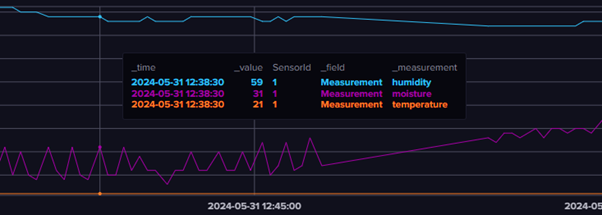
\includegraphics[width=\textwidth]{images/Graph.png}
\caption{Diagramm der Werte eines neuen Gerätes. (Licht wurde aus optischen Gründen entfernt) \cite{lameres1998fuzzy}}
\label{fig:Fuzzy Voltage Controller}
\end{figure}

\subsection{Umgesetzte Funktionen}
Momentan verbindet sich ein neues Gerät automatisch mit dem System; weitere Angaben des Nutzenden sind nicht nötig. Jede Minute werden Sensorendaten gesendet, welche in einer Datenbank gespeichert werden. Alle 5 Minuten werden die Werte überprüft. Ein Logger stellt fest, wenn Werte nicht optimal sind und eine Pumpe wird eingeschaltet, falls der Boden der Pflanze zu trocken ist. Der Nutzende kann sich nach aktuellen Informationen über die Pflanze erkundigen.

Die Grundfunktionen sind hiermit umgesetzt, es bleiben jedoch noch viele weitere Funktionen offen, um ein für den Endkunden fertiges Produkt zu erstellen. Der Kunde sollte die Pflanzenart wählen können und mehrere Optionen haben, wie er mit dem Gerät interagieren möchte. Der Sprachassisstent ist bisher lediglich rudimentär eingebunden, er könnte Warnungen geben, falls sich Werte außerhalb des optimalen Bereichs bewegen oder dem Nutzer verschieden Möglichkeiten geben das System anzupassen: Beispielsweise die Pumpe auszustellen, Zeitabstände festzulegen, die Pflanzenart zu ändern oder neue optimale Werte eingeben.

Hierfür, und für die Einbindung der Machine Learning - Algorithmen müssen weitere Datenbanken erschaffen werden, welche die optimalen Werte einer Pflanzengattung für jede spezielle Pflanze anpassen kann. Momentan exisitert nur eine statische CSV-Datei, Änderungen würden alle Pflanzen betreffen.

\subsection{Qualität des Codes}
Generell wäre Java für einen Großteil des Codes eine bessere Entscheidung gewesen.\cite{intellectsoft2023java} 

Durch den Fokus auf Klassen, wie etwa die optimale und echte Pflanze, wären klar gekennzeichnete Typen und Kompilierung von Vorteil gewesen. Java ist bei großen Projekten stabiler und Probleme bei der Kommunikation zwischen den Klassen sind schneller ersichtlich. Auch ist Threading bei Python um einiges unstabiler, Multithreading wird überhaupt nicht unterstützt. 

Zur Einschätzung des Codes wird das Lean-Modell, unterteilt in sieben Schritte, benutzt.\cite{lutkevich2024lean}

\begin{itemize}
    \item Verschwendung minimieren: Regelmäßig wurde im Projekt nicht mehr genutzter Code gelöscht, anstatt ihn zu behalten oder zu kommentieren. Keine Funktion benutzt mehr Parameter als sie benötigt und gibt nur die für sie relevanten Werte zurück.
    \item Fokus auf Qualität: Funktionen wurden mithilfe von Cucumber erstellt, um Nutzen für den Kunden zu schaffen. Jede Funktion musste einen Mehrwert für den Kunden bringen, Ziel war es nicht ein theoretisches System zu erschaffen, sondern eines, welches in jedem Schritt den Kunden weiterbringt.
    \item Lerneffekte: Lerneffekte wurden durch die regelmäßige Absprache mit der Betreuerin verstärkt. Bei verschiedenen Technologien wurden die Vor-und Nachteile besprochen.
    \item Späte Festlegung: Vor der finalen Implementierung wurden die Technologien ausgiebig getestet, um ihre Grenzen und Möglichkeiten zu verstehen. Manche Sensoren hatten eingebaute Bibliotheken, um händische Rechnungen zu vermeiden. Ebenso bietet die NoSQL-Sprache von Influx viele Möglichkeiten in der Anfrage bereits die richtigen Ergebnisse zu erhalten, ohne aufwendige Rechnungen durchzuführen.
    \item Schnelle Lieferung: Es wurden kleine Iterationszeiten gewählt, um Fehler möglichst schnell zu erkennen und Gegenwert für den Kunden zu schaffen. Alle ein bis zwei Wochen wurde eine neue Version deployed. So war das System schon früh aktiv und lief ununterbrochen auf dem Server. Der Nutzen für den Kunden - die Pflanze am Leben zu halten - konnte so bereits früh erfüllt werden.
    \item Respekt vor Arbeitenden: Durch regelmäßige Rücksprachen mit dem Betreuen wurde sichergestellt, dass sich das Projekt jederzeit im Zeitrahmen befindet, und Ziele sinnvoll gesetzt werden. So konnte mit ausreichend Zeitpuffern gearbeitet werden.
    \item Optimierung: Durch den Fokus auf Cucumber und Unit Tests stand Optimierung von Anfang an im Vordergrund. Änderungen im Code und Fehler wurden so früh erkannt.
\end{itemize}

Generell wurden  Klassen und Module möglichst klein gehalten. Ein Interface-Ansatz für die optimale und echte Pflanze erscheint im ersten Moment sinnvoll, bis auf ihre reale Repräsentation haben die beiden jedoch kaum etwas gemeinsam. Während die echte Pflanze auf eindeutigen Werten beruht, gibt die Optimale lediglich Richtlinien vor. So haben die beiden Klassen keine übereinstimmenden Attribute und es wurde sich dafür entschieden zwei gänzlich voneinander getrennte Klassen zu benutzen.

\subsection{Tauglichkeit des Mikrocontrollers und der Sensoren}
Sowohl der Microcontroller als auch der Großteil der Sensoren sind für das Projekt geeignet.

Mithilfe der Arduino-Infrastruktur konnten externe Technologien leicht in das Projekte miteingebunden werden, der Arduino selbst wies nur Probleme bei der Internetverbindung auf. Für einen ersten Prototyp erwies sich der Microcontroller als ideal, wenn auch etwas zu leistungsfähig. Für spätere Builds reicht ein billigerer Microcontroller mit weniger Anschlüssen und einer geringeren Rechenfähigkeit aus. Der Microcontroller, ein Renesas RA4M1, arbeitet mit einer Taktung von 48MHz und 32kb Ram. Für einen nächsten Prototypen sollte der Controller zurückgestuft werden, beispielsweise für einen FA0E1, mit lediglich 32MHz. Dieser runtergeschraubte Controller sollte für die einfachen Berechnungen des Projektes ausreichend sein.

Die Sensoren blieben über den gesamten Einsatz stabil und gaben keine Fehler. Die Ergebnisse waren genau und konnten einfach übersetzt werden. Lediglich der Bodenfeuchtigkeitsmesser, welcher arbiträre Werte benutzt ist zu ungenau. Hier wäre ein anderer Sensor von Vorteil, dass alle Geräte die selben Werte produzieren. Ein geeichter Tensiometer ist hier sinnvoll, wie etwa der HYG EFS-10.\cite{reichelt2024hygefs10}

\subsection{Skalierung}
Da bisher keine weiteren Geräte an das System angeschlossen wurden sind konnte das System nicht exakt getestet werden. Jedoch konnten mit einem Dummy-Sender Daten über MQTT geschickt werden, um zu testen wie sich die Technologien bei einem Vielfachen der Daten verhalten.

Durschnittlich benötigt das Senden einer MQTT-Nachricht mit einem Dummy-Sender etwa 0.07 Sekunden. Dies ergibt etwa 850 Nachrichten pro Minute.

\begin{verbatim}
    Published 83 to light_ard in 0.066460 seconds
    Published 99 to moisture_ard in 0.081350 seconds
    Published 74 to humidity_ard in 0.084083 seconds
    Published 44 to temperature_ard in 0.078810 seconds
\end{verbatim}

Der Sender konnte zwanzigmal gestartet werden, ohne dass Probleme beim Main-Controller entstehen. Ein echtes Gerät sendet 48 Nachrichten pro Minute. Es können mit diesen Technologien jetzt bereits etwa 350 Geräte verbunden werden. Beim Öffnen von weiteren Sendern kam es zu Problemen auf der Sendereinheit, nicht beim Controller.

Die Daten konnten von Influx ohne Komplikationen verarbeitet werden.

\begin{figure}[H]
\centering
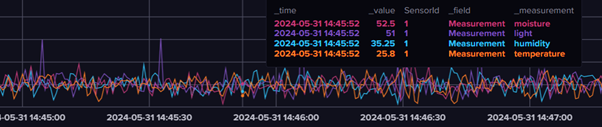
\includegraphics[width=\textwidth]{images/stresstest.png}
\caption{Diagramm der zufallsgenerierten Werte der Dummy-Sender. \cite{lameres1998fuzzy}}
\label{fig:Fuzzy Voltage Controller}
\end{figure}

Anhand dieser Daten kann man davon ausgehen, dass sowohl MQTT, als auch InfluxDB imstande sind das System sinnvoll zu skalieren und für den Produktionsbetrieb eingesetzt werden können.
